\documentclass{beamer}
\usepackage[utf8]{inputenc}
% sleak blue theme
\usetheme{Madrid}

\title[	Threats and security of cryptocurrencies]
{Threats and security of cryptocurrencies}
\subtitle{A story told short}
 
\author[Łukasz Klasiński] 
{ Łukasz Klasiński}
 
\institute[UWr]
{
  IT department of\\
  University of Wrocław
}

\date[18-12-2018]
{Blockchain and it's applications}
 

\begin{document}
 
\frame{\titlepage}
\begin{frame}
    \frametitle{Agenda}
      \tableofcontents
\end{frame}


\section{Threats of cryptocurrency market}
\begin{frame}
\frametitle{Threats of cryptocurrency market}
\begin{itemize}
    \item<1-> Value of currency
    \begin{itemize}
        \item<2-> no organizations controlling market and no inflation 
        \item<3-> determined by value of transactions made by participants
        \item<4-> loss of confidence may result in collapse of trading activities and value
        \item<5-> liquidity concerns
    \end{itemize}
    \vspace{20pt}
    \begin{block}{Strategy}<6->
         Mining companies try to avoid exceeding the 51\% confidence limit in order
         to make value of cryptos more stable  
    \end{block}    
    \begin{exampleblock}{Example}<7->
        \textbf{GHash.IO} bitcoin mining pool exceeded 51\% pool threshold in July 2014.  
    \end{exampleblock}
\end{itemize}
\end{frame}

\begin{frame}
\frametitle{Threats of cryptocurrency market}
\begin{itemize}
    \item<1-> Operational risks
    \begin{itemize}
        \item<2-> not possible to reverse transactions
        \item<3-> access to monies not possible after loosing keys
        \item<4-> can't block/stop crypto wallet after loosing keys
    \end{itemize}
    \vspace{20pt}
    \begin{block}{Strategy}<5->
        Keeping backup of your keys, encrypting them, splitting monies into multiple 
        wallets
    \end{block}
\end{itemize}
\end{frame}

\begin{frame}
\frametitle{Threats of cryptocurrency market}
\begin{itemize}
    \item<1-> Regulatory risks
    \begin{itemize}
        \item<2-> some countries may prevent use of cryptocurrencies
        \begin{itemize}
            \item<3-> no control over taxes paid per transactions
            \item<4-> government doesn't like decentralized things
            \item<5-> government depend on 'real' monies (that are outranked by crypto)
            \item<6-> transactions may break anti-money laundering regulations
        \end{itemize}
    \end{itemize}
\end{itemize}
\vspace{20pt}
\begin{exampleblock}{Currently banned in}<7->
    Algeria, Egypt, Morocco, Canada(banking), Bolivia, Columbia, Ecuador, Saudi Arabia, Iran, Bangladesh,
    India(banking), Nepal, Pakistan, China, Taiwan, Cambodia, Indonesia, Thailand(banking), Vietnam.
\end{exampleblock}
\end{frame}

\begin{frame}
    \frametitle{Threats of cryptocurrency market}
    \begin{itemize}
     \item<1-> Cyber risks
     \begin{itemize}
        \item<2-> tempting target for hackers and criminals
        \item<3-> viruses that drain crypto wallets and steals crypto
        \item<4-> investors must rely on their own security or third parties 
        \item<5-> cryptocurrency is highly reliant upon unregulated companies, including some 
        that may lack appropriate internal controls and may be more susceptible to fraud and theft 
        than regulated financial institutions
        \item<6-> the software needs to be regularly updated and suspect at times
     \end{itemize}
    \end{itemize}
\end{frame}
\begin{frame}
\frametitle{Threats of cryptocurrency market}
    \begin{itemize}
        \item<1-> Market risks
        \begin{itemize}
            \item<2-> currency trades only on demand
            \item<3-> finite amount of the currency 
            \item<4-> limited ownership may make it susceptible to market manipulation
            \item<5-> more volatile than other physical currencies
        \end{itemize}
    \end{itemize}
\end{frame}
\begin{frame}
\frametitle{Threats of cryptocurrency market}
    \begin{itemize}
        \item<1-> Risks for business
        \begin{itemize}
            \item<2-> costs involved in mitigation 
            \item<3-> anti-money laundering and privacy laws problems with global range
            \item<4-> individuals can seek to circumvent tax regulations 
            \item<5-> liquidity concerns (again)
            \item<6-> transaction fees
        \end{itemize}
    \end{itemize}
\vspace{20pt}
\begin{exampleblock}{Example}<7->
    After about year and a half Steam ended support for bitcoin payments because of
    'hight fees and volatility' of a bitcoin.
\end{exampleblock}
\end{frame}

\section{Future threats}
\begin{frame}
\frametitle{Future threats}
    \begin{itemize}
        \item<1-> Energy consumption(bitcoin)
        \begin{itemize}
            \item<2-> currently using 45TWh which is just greater then Portugal(52th in the world)
            \item<3-> record use is estimated about 73TWh (just greater then Austria ranked 39th)
            \item<4-> currently estimated cost of electricity of  mining one bitcoin higher then value of bitcoin (4000\$ vs 3100\$) 
            \item<5-> with electricity production costs rising and banning crypto mining in electricity-cheap countries (like China), mining may be unprofitable                    
        \end{itemize}
    \end{itemize}
\end{frame}
\begin{frame}
\frametitle{Future threats}
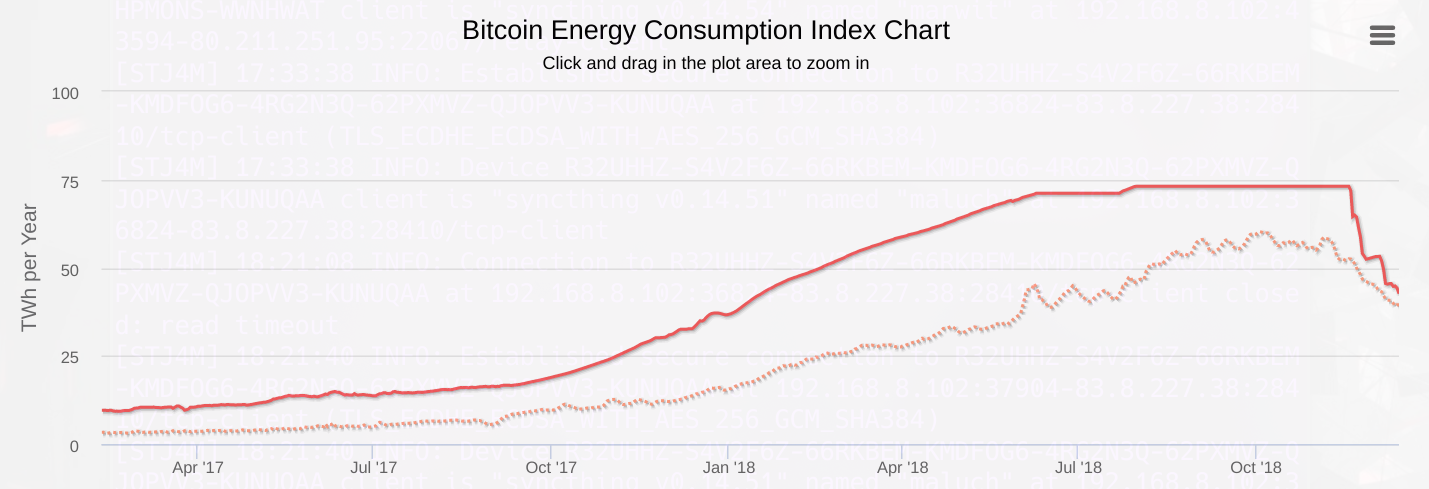
\includegraphics[width=\textwidth]{elec_chart.png}<1>
\begin{itemize}
    \item<2-> Scalability(bitcoin)
        \begin{itemize}
            \item<3-> capacity is limited by block creation time of 10min
            \item<4-> results in estimated 3-7 transactions per second
            \item<5-> creates bottleneck when there is more then 3 transactions per second
            \item<6-> results in transaction fees skyrocketing and delayed processing of transactions
            \item<7-> block size limit problem
        \end{itemize}
\end{itemize}
\end{frame}
\begin{frame}
\frametitle{Future threats}
    \begin{itemize}
        \item<1-> Node distribution
        \begin{itemize}
            \item<2-> full and half nodes miners
            \item<3-> half nodes more preferable
            \item<4-> unequal distribution of full nodes
            \item<5-> problem with data propagation
            \item<6-> overloaded full nodes
        \end{itemize}
    \end{itemize}
\end{frame}
\begin{frame}
\frametitle{Future threats}
    \begin{itemize}
        \item<1-> Quantum computing
        \begin{itemize}
            \item<2-> private key vulnerable to quantum algorithms
            \item<3-> new methods of authentications would be needed
            \item<4-> 'quantum safe cryptography' is the only hope 
            \item<5-> some crypto claims to be 'quantum-safe' (NEO)
        \end{itemize}
    \end{itemize}
\end{frame}
\begin{frame}
\frametitle{Future threats}
    \begin{itemize}
        \item<1-> Bubble
        \begin{itemize}
            \item<2-> numerous experts in economics identify cryptocurrencies as 'economic bubbles'
            \item<3-> e.g Paul Krugman, Robert J. Shiller, Joseph Stiglitz etc.
            \item<4-> 'newbies' to crypto markets may loose absurd amount of money because of 'bubbles'
            \item<5-> includes drops even by 80\%(September 2018, MVIS, top 10 crypto)
        \end{itemize}
    \end{itemize}
\end{frame}
\begin{frame}
\frametitle{Future threats}
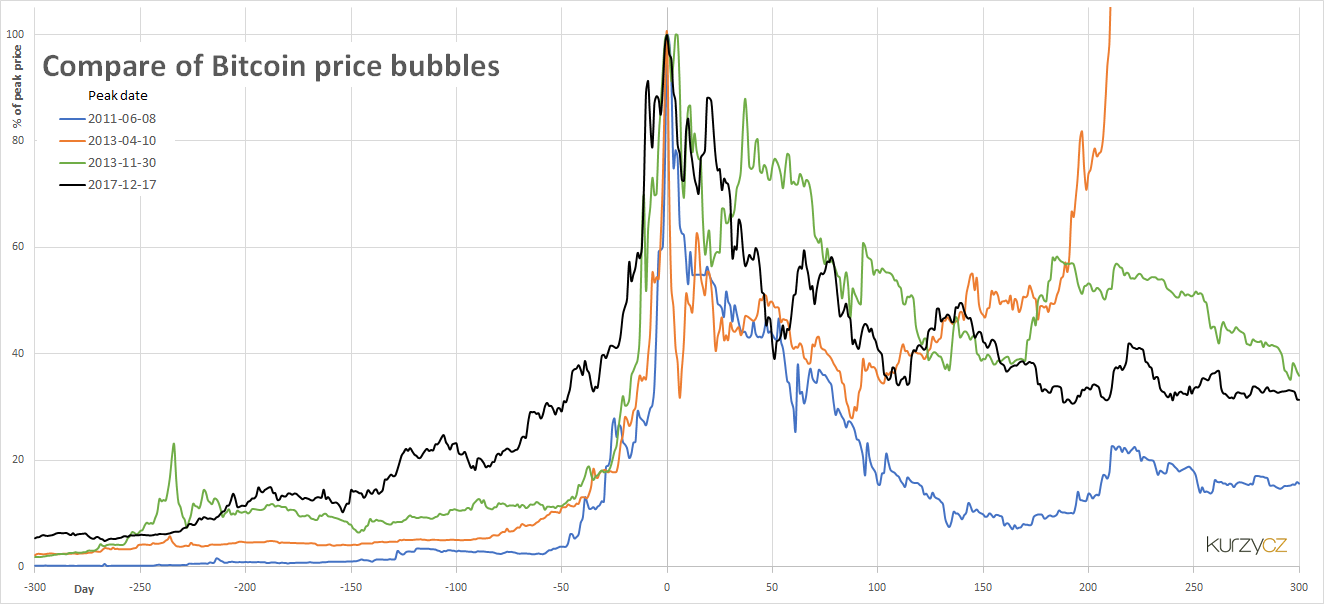
\includegraphics[width=\textwidth]{bubble-chart.png}<1>
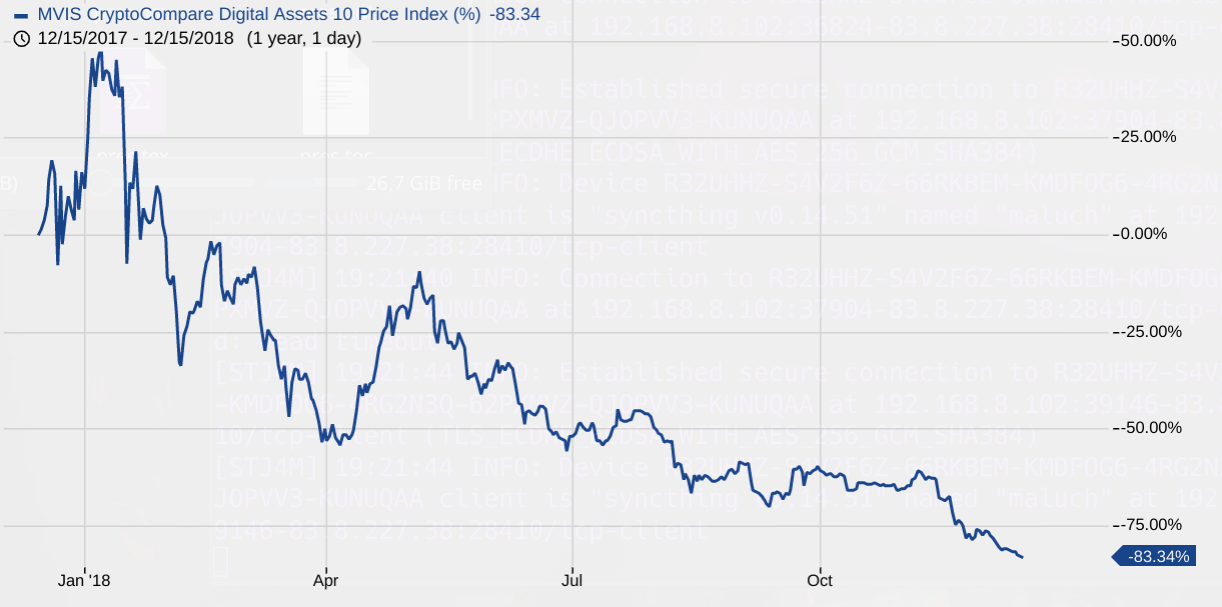
\includegraphics[width=\textwidth]{mvis-chart.png}<2>
\end{frame}

\section{Cryptocurrency in crime}
\begin{frame}
\frametitle{Cryptocurrency in crime}
    \begin{itemize}
        \item<1> Medium of exchange
        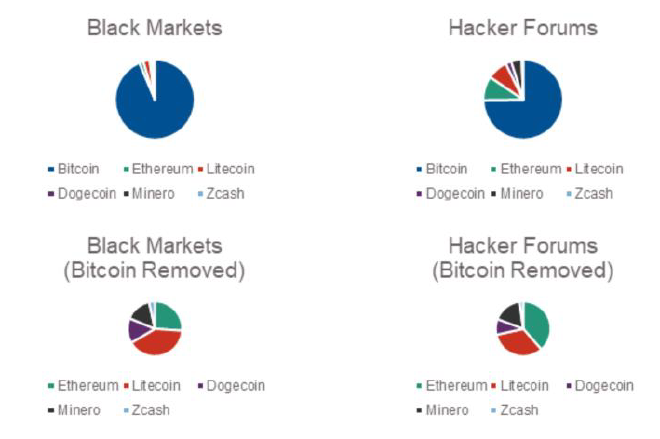
\includegraphics[width=100mm]{exchange-chart.png}<1>
    \end{itemize}
\end{frame}
\begin{frame}
    \frametitle{Cryptocurrency in crime}
        \begin{itemize}
            \item<1-> Ransomware
            \begin{itemize}
                \item<2-> virus that encrypt data
                \item<3-> ransomware payments prefers bitcoin
                \item<4-> even if you pay it doesn't mean you'll get your data
                \item<5-> can be devastating for bigger companies 
            \end{itemize}
        \end{itemize}
\end{frame}
\begin{frame}
    \frametitle{Cryptocurrency in crime}
        \begin{itemize}
            \item<1> e.g Thanatos(2018)
            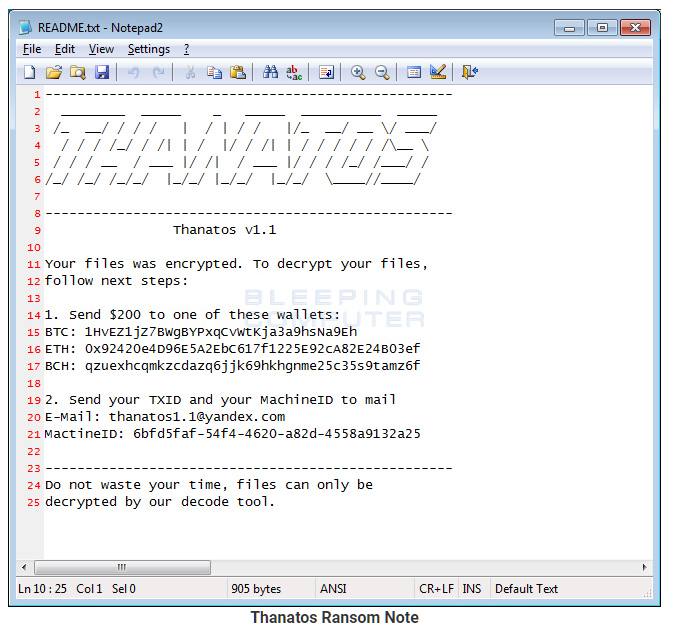
\includegraphics[width=80mm]{thanatos-chart.png}<1>
        \end{itemize}
\end{frame}
\begin{frame}
    \frametitle{Cryptocurrency in crime}
        \begin{itemize}
            \item<1-> Cryptojacking
            \begin{itemize}
                \item<2-> prefers monero
                \item<3-> can be mined on CPUs
                \item<4-> better privacy then bitcoin
                \item<5-> originally people running miners on company hardware
                \item<6-> evolved to worms dropping miners
                \item<7-> possible in browser(using JavaScript)
                \item<8-> hacking routers to insert code into https
                \item<9-> possible on android systems
                \item<10-> 4000\% increase in 2018 
            \end{itemize}
        \end{itemize}
        \begin{exampleblock}{Example}<11->
            Few weeks ago security firm Radiflow announced discovery of crypto mining
            malware in the monitoring network of water utility in Europe.
        \end{exampleblock}                
\end{frame}    
\begin{frame}
    \frametitle{Cryptocurrency in crime}
        \begin{itemize}
            \item<1> e.g Worms
            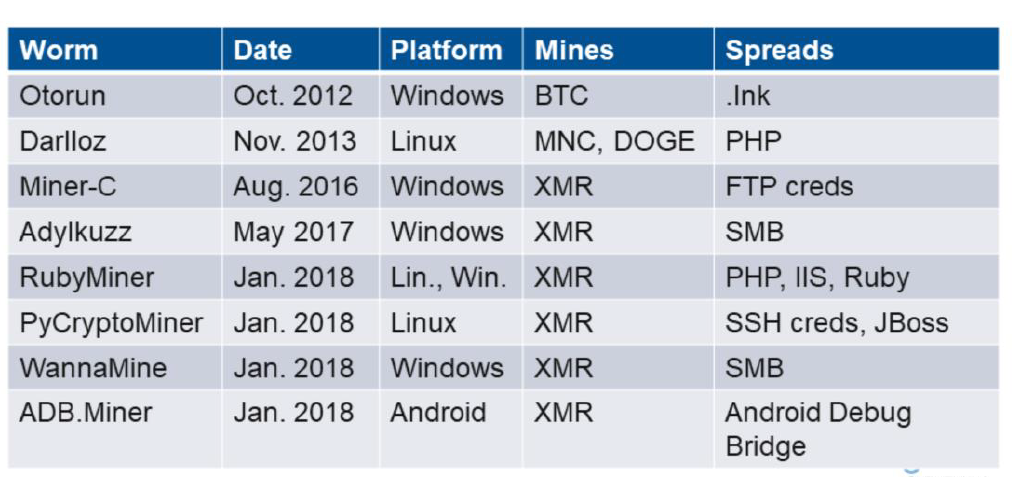
\includegraphics[width=100mm]{worms-chart.png}<1>
        \end{itemize}
\end{frame}
\begin{frame}
    \frametitle{Cryptocurrency in crime}
        \begin{itemize}
            \item<1-> Thieft
            \begin{itemize}
                \item<2-> Wallets using vishing, smishing etc.
                \item<3-> Exchanges
                    \begin{itemize}
                        \item<4-> Mt. Gox,   2014 \$450M in BTC
                        \item<4-> Bitfinex,  2016 \$72M  in BTC
                        \item<4-> Coincheck, 2018 \$530M in NEM
                    \end{itemize}
                \item<5-> Tor proxy address rewrites \$22K
                \item<6-> Flaws in smart contracts
                \item<7-> Threat mails
            \end{itemize}
        \end{itemize}
\end{frame}
\section{Frauds \& Scams}
\begin{frame}
    \frametitle{Frauds \& Scams}
        \begin{itemize}
            \item<1-> Initial Coins Offerings(ICO)
                \begin{itemize}
                    \item<2-> Prodeum - fruit and veggies track system on Etherium blockchain (\$2.4K)
                    \item<3-> PlexCoin - new cryptocurrency promising hight gains for inverstors (\$15M)
                    \item<4-> AriseBank - 'New revolutional way of banking' (\$4M) 
                    \item<5-> PonziCoin - cryptocurrency made and presented as scam, still earns \$250K
                \end{itemize} 
            \end{itemize}
            \begin{center}
            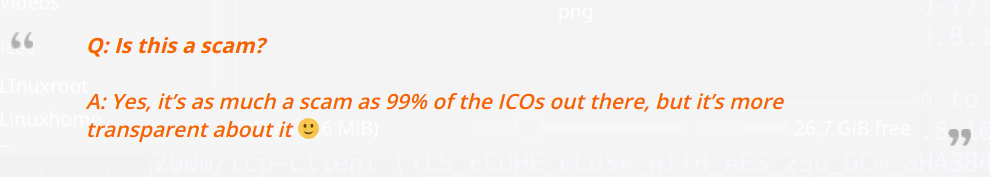
\includegraphics[width=\textwidth]{ponzed.png}<6->     
            \end{center}         
\end{frame}

\begin{frame}
    \frametitle{Frauds \& Scams}
    \begin{itemize}
        \item<1-> Ponzi schemes
        \begin{itemize}
            \item<2-> My Big Coin - same story(\$1.1M)
            \item<3-> CabbageTech - virtual currency trading advice(\$1.1M)
            \item<4-> Bitconnect - alt-coin with wallet interest
        \end{itemize}
        \begin{center}
            
\includegraphics[width=80mm]{connect.jpeg}<5->
        \end{center}        
    \end{itemize}
\end{frame}

\begin{frame}
    \frametitle{Frauds \& Scams}
    \begin{itemize}
        \item<1-> Pump-n-dump with bots
        \begin{itemize}
            \item<2-> bot usage in crypto
            \item<3-> auto selling/buying when price fell below a certain point
            \item<4-> can cause dramatic drop in price for a few sec
            \item<5-> in 2013 Markus and Willy bots caused bitcoin spike from \$150 to \$1000 over 60 days by trading with bitcoins they didn't own
        \end{itemize}
    \end{itemize}
    \vspace{10pt}
    \begin{exampleblock}{Example}<6->
        In 2017 price of Etherium dropped to 10 cents for few sec, causing bots to cascade sell. The cause was a multi\-million sell order on the exchange.   
    \end{exampleblock}     
\end{frame}

\begin{frame}
    \frametitle{Mining strategies}
    \begin{itemize}
        \item<1-> Temporary block withholding 
        \begin{itemize}
            \item<2-> miner (or pool) try to withhold mined valid block byt submit partial share
            \item<3-> holding valid blocks won't increase difficulty of mining puzzle
            \item<4-> can earn profits only for large miner or big pools
            \item<5-> can be detected but also easly obfuscated
        \end{itemize}
        \vspace{10pt}
        \begin{block}{Strategy}<6->
            Mine valid block, as long as block chain has one less block then you, mine new blocks.
            When main block catches up to you(off by one block) publish your blocks, making your chain the longest
            and becoming new main root.
        \end{block}     
    \end{itemize} 
\end{frame}

\begin{frame}
    \frametitle{Mining strategies}
    \begin{itemize}
        \item<1-> Majority miner 
        \begin{itemize}
            \item<2-> with majority of computation power can collect all mining rewards
            \item<3-> just ignore all other blocks and build your own chain
            \item<4-> it would be statistically always the longest one
            \item<5-> can ignore/censor chosen transactions 
            \item<6-> can become by colluding of smaller miners and emulating majority miner strategy
        \end{itemize}   
    \end{itemize} 
\end{frame}

\begin{frame}
    \frametitle{Mining strategies}
    \begin{itemize}
        \item<1-> Maintaining exchange rates
        \begin{itemize}
            \item<2-> some non-compilant strategies that affect stability in a visible way might undermine public confidence
            \item<3-> causing weaken demand for bitcoins in the short run
            \item<4-> strategies that can quickly earn many bitcoins are likely to crash exchange rate once discovered
            \item<5-> and it's difficult to cash out before crash given the liquidity limits
            \item<6-> so the strategy is to do not use unfair strategies and try to prevent others from using them
            \item<7-> since most big miners have capital tied up to mining hardware which will loose value if exchange rate declines
        \end{itemize}   
    \end{itemize}
\end{frame}

\begin{frame}
    \frametitle{Mining strategies}
    \begin{itemize}
        \item<1-> Goldfinger attack
        \begin{itemize}
            \item<2-> really just a majority miner strategy but with bad intentions
            \item<3-> attacker wish to damage given cryptocurrency stability can just buy 51\%(or redirect his own) of computing power
            \item<4-> then he can easly cause side effects of major miner strategy
            \item<5-> practically impossible on bigger players(like bitcoin, etherium), but possible on smaller ones
            \item<6-> have beed observed through altcoin infanticide on CoiledCoin in 2012 (rip)
        \end{itemize}   
    \end{itemize}
\end{frame}

\begin{frame}
    \frametitle{Mining strategies}
    \begin{itemize}
        \item<1-> Feather-forking
        \begin{itemize}
            \item<2-> strategy that can blacklist given addresses
            \item<3-> publicly promise that if target address is in certain block, miner ignores it and attempt to create fork
            \item<4-> the attacker fork will continue until it outraces main branch or falls by $k$ blocks, at which point attacker will concede
            \item<5-> on expectation an attacker with $\alpha \le 50\%$ of the mining power will loose monies but will succeed in blocking blacklisted transaction with positive probability
            \item<6-> attacker convince others to join by rasing fee necessary to commit a "blacklisted" transaction to $\alpha*U$, where $U$ is the average reward from a block
        \end{itemize}   
    \end{itemize}
\end{frame}

\section{Anonymity \& privacy}
\begin{frame}
    \frametitle{Anonymity \& privacy}
    \begin{itemize}
        \item<1-> Deanonymization
        \begin{itemize}
            \item<2-> in most crypto addresses are public when making transaction
            \item<3-> so a seller can check amount of monies on buyers addresses
            \item<4-> same with companies and mining pools
            \item<5-> it is also possible to trace flow of monies and conclude addresses that belong to the same individuals
            \item<6-> one way to prevent it (seller) is to link every transaction to new address
            \item<7-> by contrast customer may need to assemble payment amount from multiple addresses he owns
            \item<8-> identification of regular user address may be possible for authorities since most data pass through providers
        \end{itemize}
        \begin{exampleblock}{Example}<9->
            \textbf{Chainalysis} is a company specializing in connecting crypto addresses to real identities and other analysis over blockchains. They work with governments to 
            find identities of criminals.
        \end{exampleblock}             
    \end{itemize}    
\end{frame}

\begin{frame}
    \frametitle{Anonymity \& privacy}
    \begin{itemize}
        \item<1-> Improving anonymity
        \begin{itemize}
            \item<2-> \textbf{Coin-Join}
            \item<3-> User wanting to perform transaction seek for others
            \item<4-> They combine their transaction into one 'big' with inputs corresponding to their addresses
                        and outputs to recipients
            \item<5-> Thanks to that there is no way to map inputs to outputs
            \item<6-> User can benefit without others using multiple accounts
            \item<7-> and u cant be sure if those aren't other users
            \item<8-> in practice need dedicated servers to create merged transactions 
            \item<9-> newest protocol don't allow participants to know what addresses are at inputs
        \end{itemize}   
    \end{itemize}
    \begin{center}
    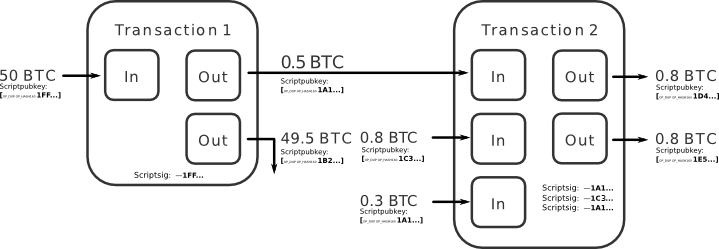
\includegraphics[width=80mm]{coin-join.png}<9->   
    \end{center} 
\end{frame}

\begin{frame}
    \frametitle{Anonymity \& privacy}
    \begin{itemize}
        \item<1-> Improving anonymity
        \begin{itemize}
            \item<2-> \textbf{Mixcoin}
            \item<3-> multiple users send monies to one pot
            \item<4-> then they receive back the same amount from coins submitted by other users of the mix onto new address
            \item<5-> this provides anonymity toward external entities
            \item<6-> there are many existing services that do it for small fee 
        \end{itemize}   
    \end{itemize}
\end{frame}

\begin{frame}
    \frametitle{Anonymity \& privacy}
    \begin{itemize}
        \item<1-> Improving anonymity
        \begin{itemize}
            \item<2-> \textbf{Zerocoin}
            \item<3-> extension to bitcoin protocol that improves bitcoin anonymity
            \item<4-> allows conversion of non-anonymous bitcoins to secure, anonymous zerocoins
            \item<5-> presentation topic material?
        \end{itemize}   
    \end{itemize}
\end{frame}

\section{Security layers of crypto}
\begin{frame}
    \frametitle{Security layers of crypto}
    \begin{itemize}
        \item<1-> How to choose cryptocurrency?
        \begin{itemize}
            \item<2-> divide it into layers
            \item<3-> decide what is most important to you
            \item<4-> choose!
        \end{itemize}   
    \end{itemize}
\end{frame}

\begin{frame}
    \frametitle{Security layers of crypto}
    \begin{itemize}
        \item<1-> The First layer: Coins and Tokens
        \begin{itemize}
            \item<2-> When choosing cryptocurrency you are taking all the risks of the protocol
            \item<3-> if someone finds flaws in protocol they can compromise entire network
            \item<4-> find out if it can be centralized. E.g. in case of bitcoin it is centralized around few biggest mining pools. This means
                that if they cooperate, they can compromise entire network
            \item<5-> look at the genesis - who holds what
            \item<6-> be aware of etherium based ICOs and possible roll backs from founders
        \end{itemize}   
    \end{itemize}
\end{frame}

\begin{frame}
    \frametitle{Security layers of crypto}
    \begin{itemize}
        \item<1-> The Second layer: Exchanges
        \begin{itemize}
            \item<2-> exchange services are written in custom code with infrastructure security that has nothing to do with blockchain
            \item<3-> so the most important is trust and credibility
            \item<4-> a lot of exchanges started business recently and didn't invest into proper security measures
            \item<5-> ...but if someone steals monies from an exchange it's almost impossible to do anything about it
            \item<6-> it's best to check the security part of exchange websites
        \end{itemize}   
    \end{itemize}
\end{frame}

\begin{frame}
    \frametitle{Security layers of crypto}
    \begin{itemize}
        \item<1-> The Third layer: Wallet
        \begin{itemize}
            \item<2-> Hot wallet
            \item<3-> Cold wallet
        \end{itemize}   
    \end{itemize}
\end{frame}

\begin{frame}
    \frametitle{Fin}
    \begin{center}
    Thanks for your attention!
    \end{center}
\end{frame}


\end{document}